\documentclass[12pt]{article}

\usepackage{lmodern}	% for nice Fonts
\usepackage{graphicx}	% For adding pictures
\usepackage[font=small,labelfont=bf]{caption}  % Caption formatting
\usepackage{subcaption}

\usepackage{hyperref}


%for editing purposes
\usepackage{color}

\title{Curly-Squeegee Process Book}
\author{ Brian Kimmig \& Jimmy Moore}
\date{\today}


\begin{document}
\maketitle

\begin{abstract}
	Curly-Squeegee (CS) is a web-bsaed tool for visualizing and exploring actor filmographies in an interactive way. By enabling users to search for their favorite actors and see their entire body of work displayed a variety of ways, we hope it invites them to explore the different views, select and filter different sub-sets of actor filmography data, and find intersting or surprising hidden trends.
\end{abstract}

\tableofcontents

\newpage


\section{Editing notes}

{\color{red}

Depending on how thourough we want to be (and how much time we have for thoroughness) we could incorporate any of the talking points from the ``example" documents
\begin{itemize}
	\item \href{http://dataviscourse.net/2015/assets/process_books/bansal_cao_hou.pdf}{Real time audio visualization project - Soundscapes}
	\item \href{http://dataviscourse.net/2015/assets/process_books/walsh_trevino_bett.pdf}{Oh Shit, earthquakes!}
\end{itemize}

Options include:
\begin{enumerate}
	\item Explicit analysis on color choices, modes of comparison (length, hue, etc)
	\item in-depth explanation of our  choice of design principles or encodings \textbackslash visual variables
	\item Analysis of data
\end{enumerate}
}

\newpage

\section{Project Background}

\subsection{Motivation}
	The idea for this project came from the fact that both developers watch a good amount of movies and enjoyed sites like IMDB and RottenTomatoes, but wanted something that focused on specific actors rather than being movie-centric. CS is their solution to needing to sift through lists and text to appreciate a given actors filmography. In three views, one can see their entire body of work as a timeline, with length and color encodings for film-output and film-quality, respectively, as well as career visualizations showing the breakdown of movie genre over the course of their career and a multi-axis interactive plot to explore an actors output as a function of date ranges, ratings, box office earnings, and directors.
	
	CS is meant to provide a new way of viewing actor data, and seeks to facilitiate a fun and interactive web-based solution to questions like:


	\begin{itemize}
		\item How many movies has an actor acted in?
		\item Has an actor been type-cast to a specific genre?
		\item What is the best movie they have made? The worst?
		\item Do they consistently star in well-reviewed films?
		\item Has their career had a golden period in which they were particularly busy, or appeared in well-reviewed films?
	\end{itemize}
	
\subsection{Intended Audience}
Curlee Squeege is geared towards the general public and accessible to the occasional movie-goer to film buffs, alike.  

Users are presented with a list of trending actors as well as a search box, so they can start using the tool immediately with little explanation.

We hope that the site design and visualization aesthetics make it a natural and easy tool to use.
\newpage 

\section{Data Collection}
	This application readily takes advantage of several pre-packaged movie APIs, specifically My API Films and OMdb. We have set up a web framework using node.hs and Meteor which uses a RESTful architecture to gather API calls via GET requests. We store all data in a MongoDB database. This dataset is fairly dynamic since we rely on user queries to pull the necessary information from the APIs.
	
	\begin{center}
	\color{blue}
	\textbf{Do we want to have a breakdown or description of the API call, data retrieval, and database storage? }
	\end{center}
	
\subsection{Data Processing}
	API requests are returned in JSON format, so there is little clean-up beyond. Returned data is fairly detailed, so we selectively cull certain uncessary fields and aggregate filmography data based on what we want to visualize. We have two data structures in our databases:
	
	\begin{itemize}
		\item Actor Table: This stores all the actor information of a selected actor, including the movies they've acted in.
		\item Movie Table: This contains all of the information for each movie we wish to plot or visualize.
	\end{itemize}
	
	The data collection and filtering is probably the most sophisticated portion of this project. With everything stored and readily accessible, we use built-in javascript math functions and agregate parameter counts of our actor data to illustrate actor filmographies.

\newpage 

\section{Project Evolution}

This project has had an accelerated development cycle and we quickly settled on a fixed set of views.  Details have not changed significantly from the proposal document, but we will compare and contrast any differences below.

\subsection{Landing Page}

	\begin{figure}[h!]
		\centering
		\begin{subfigure}[t]{.5\textwidth}
			  \centering
			  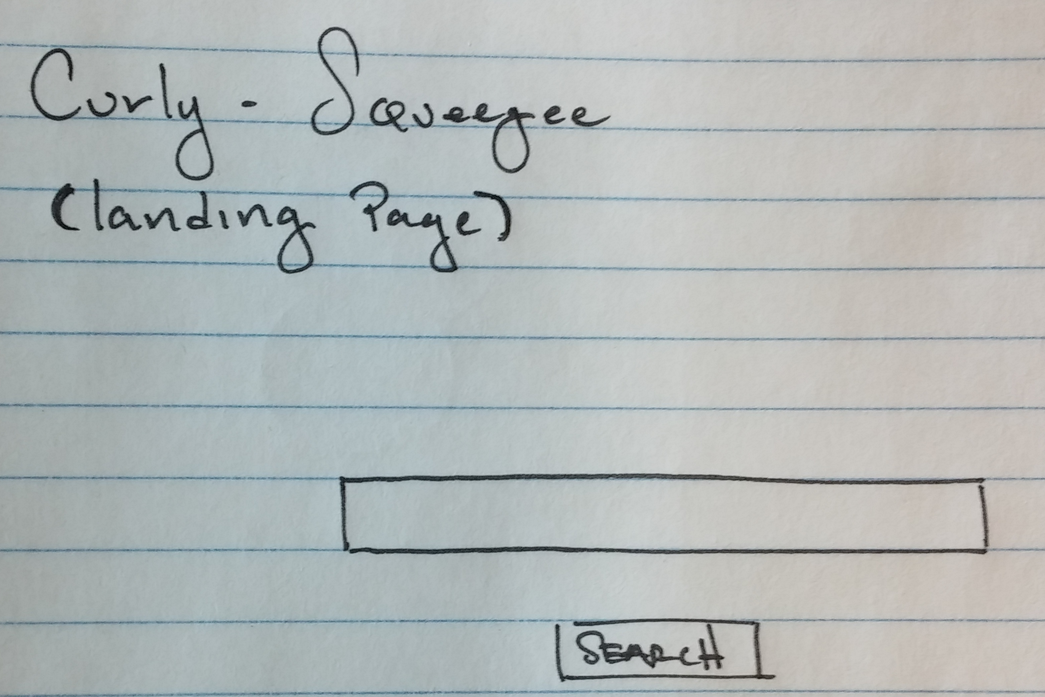
\includegraphics[width=\linewidth]{images/landingPage_crop.png}
			  \caption{Original design sketch}
			  \label{fig:sub1}
		\end{subfigure}%
		\begin{subfigure}[t]{.8\textwidth}
			  \centering
			  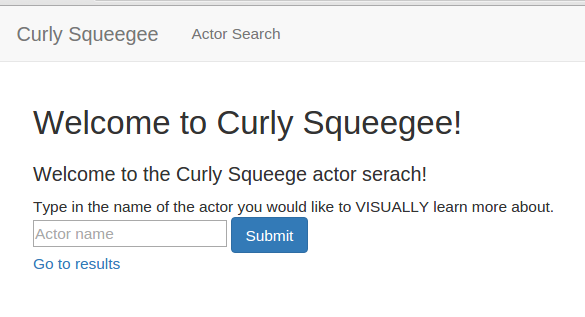
\includegraphics[width=0.75\linewidth]{images/landingPage.png}
			  \caption{Current implementation}
			  \label{fig:sub2}
		\end{subfigure}%
		\caption{Landing page development}
		\label{fig:landingPage}
	\end{figure}


\subsection{Loading Page}

			\begin{figure}[h!]
				\centering
				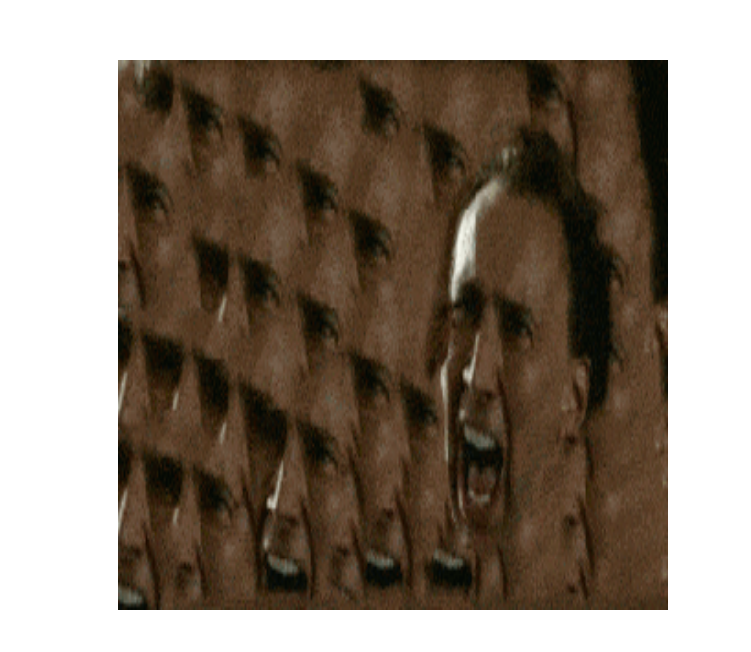
\includegraphics[scale=0.3]{images/loadingPage.png}
				\caption{Once the user submits a search query, the application waits for the API calls to complete and fetch the actor's filmography.  This can take upwards of 30 seconds}
			\end{figure}
			While the API calls are made and the film data is saved to the local database, we display a gif to indicate that the files are being loaded.

\subsection{Display\textbackslash Results Page}
Once the filmography has been loaded, we load our results page, which  shows a number of views and actor information

\subsection{Actor Fact Box}

	This data serves as an orientation tool,indicating to the user whether the correct actor was returned.  This is particularly important in cases when searching for actors with common names.  Using the OMDB API data, we are able to display a photograph of the actor, their full name, date of birth, and other derived data from the API call.  We currently display their total number of films.  other useful information would be when they started acting \textbackslash first credited role, years active, and highest or worst rated movie.
	
		\begin{figure}[h!]
			\centering
			\begin{subfigure}[t]{.5\textwidth}
				  \centering
				  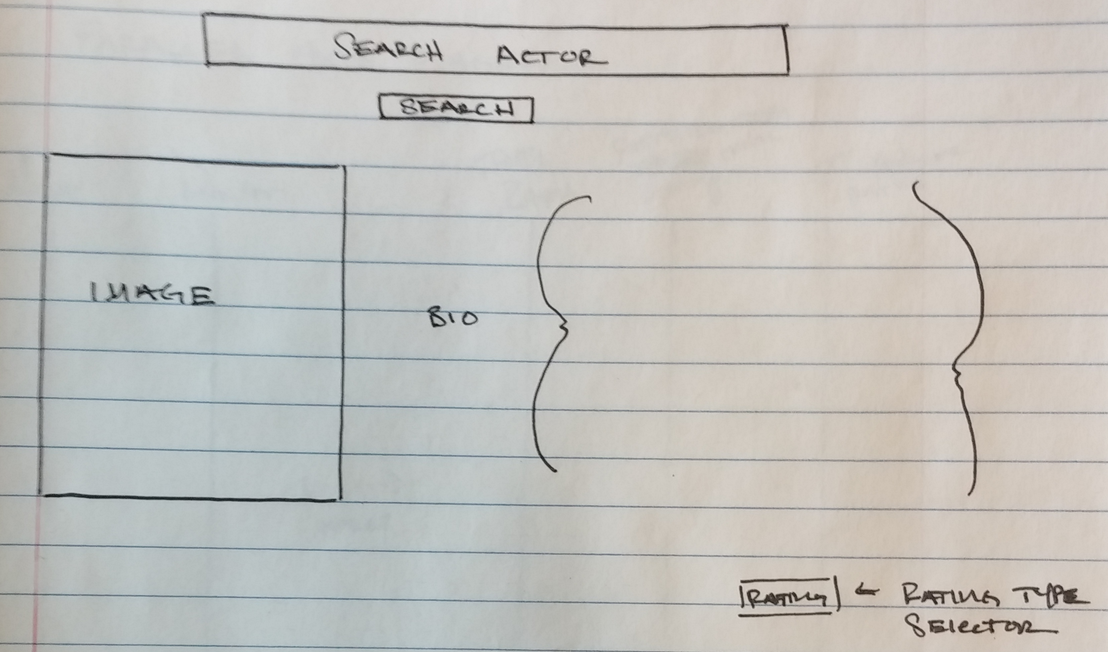
\includegraphics[width=\linewidth]{images/actorFactBox_crop.png}
				  \caption{Original design sketch}
				  \label{fig:sub1}
			\end{subfigure}%
			\begin{subfigure}[t]{.5\textwidth}
				  \centering
				  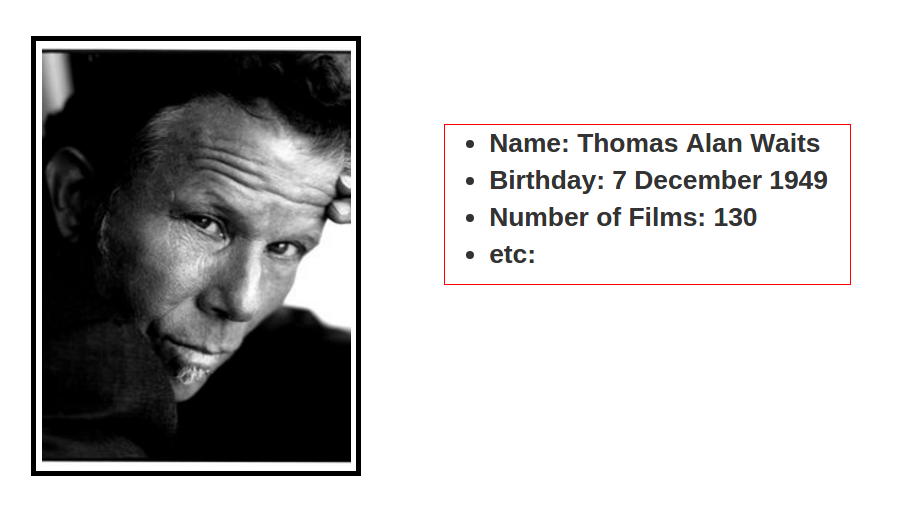
\includegraphics[width=.8\linewidth]{images/actorBox.png}
				  \caption{Current implementation}
				  \label{fig:sub2}
			\end{subfigure}%
			\caption{Actor `Fact Box' development}
			\label{fig:actorFactBox}
		\end{figure}

\subsection{Visualizations}

	Talk a bit about the different views we chose, and why.  This can be a cut/paste job from certain parts of our proposal.

\subsubsection{Filmography Timeline}

	\begin{figure}[h!]
			\centering
			\begin{subfigure}[t]{.5\textwidth}
			  \centering
			  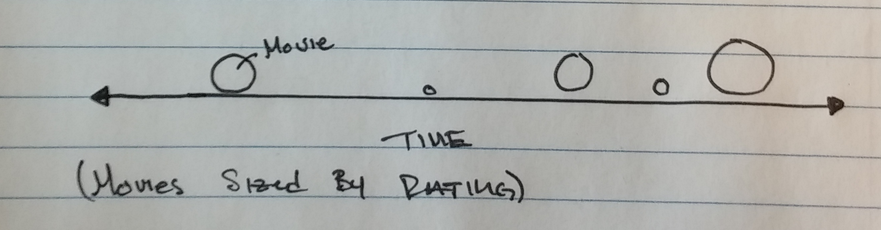
\includegraphics[width=\linewidth]{images/timeline_orig.png}
			  \caption{Original design sketch}
			  \label{fig:timelineA}
			\end{subfigure}%
			\begin{subfigure}[t]{.5\textwidth}
			  \centering
			  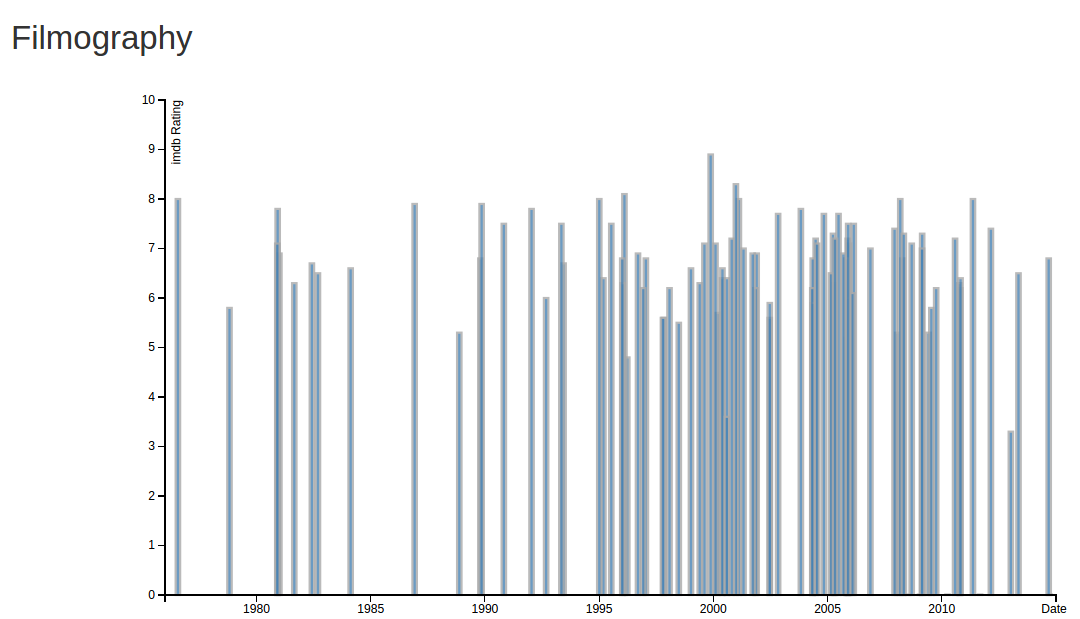
\includegraphics[width=.7\linewidth]{images/timeline_crop_waits.png}
			  \caption{First Implementation}
			  \label{fig:timelineB}
			\end{subfigure}%
			\caption{Timeline development}
			\label{fig:timeline}
		\end{figure}
		
Early in our design phase, we considered using circles on a timeline as a suitable encoding for showing film distribution.  This decision was inspired by the \href{http://mariandoerk.de/edgemaps/demo/#phils;time;;;}{philosophers, poets, and musicians} timeline comparison shown in class. The idea was to visually show the distribution (and density) of an artist's career chronologically and encode information such as film ratings or earnings as the circle radius or fill color.   This decision was later refined after our brainstorming session (Section \ref{sec:Projcet Feedback}). Concerns were raised that actors with frequent and\textbackslash or successful work would create a cluttered timeline visual.  We also recalled thelack of effectiveness with comparing quantitative values when encoded as an area, and decided it would be better to switch to a barchart visual.  This way we could cleanly show movie release dates and have a more direct comparison of ratings or other quantitative data by mapping it to bar height.

As we implemented our barchart visualization, we observed several issues relating to bar sizing, spacing, and overlap.  Consider the filmography of Tom Waits, shown in figure \ref{fig:timelineB}. We did not initially consider visualizing filmographies in the extreme cases of long acting careers, high film output, or areas of dense activity.  In each case, the sizing and spacing of the bars becomes an issue for readability and visual appeal.  Particularly frustrating, were areas where an actor would have multiple films released within a small time frame.  We tried separating these views by using thinner rectangles, adding stroke width to the bars, or introducing opacity.  We were not happy with any of these solutions and sought a better visualization method.

\begin{figure}
	\centering
	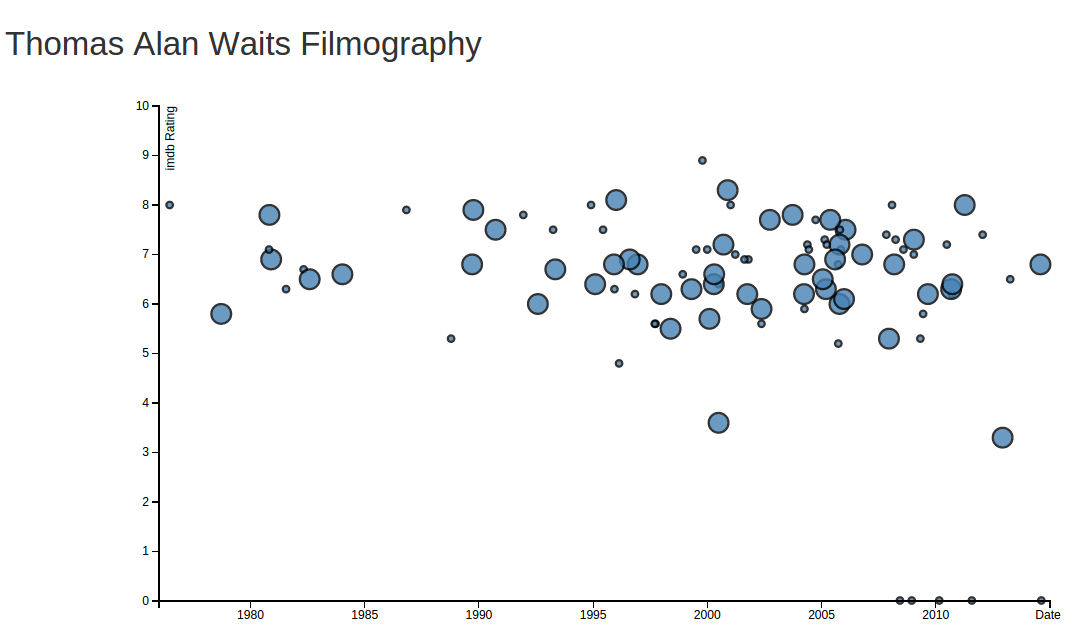
\includegraphics[width=.7\linewidth]{images/timelineC_crop_waits.png}
				  \caption{XY Plot of Tom Waits filmography.  circles are sized by number of  IMDB votes.}
\end{figure}\label{fig:xy}


Figure \ref{fig:xy} is a marked improvement over the earlier efforts to illustrate an actor's filmography.  The XY plot naturally lends itself to an ordered ranking  in each dimension, and the user can immediately identify such information as : high and low ranked films, popular films, and any trend in the actor's career over time.  For example, figure \ref{fig:deniro} verifies the slight decline of  Robert DeNiro's film quality.

\begin{figure}
	\centering
	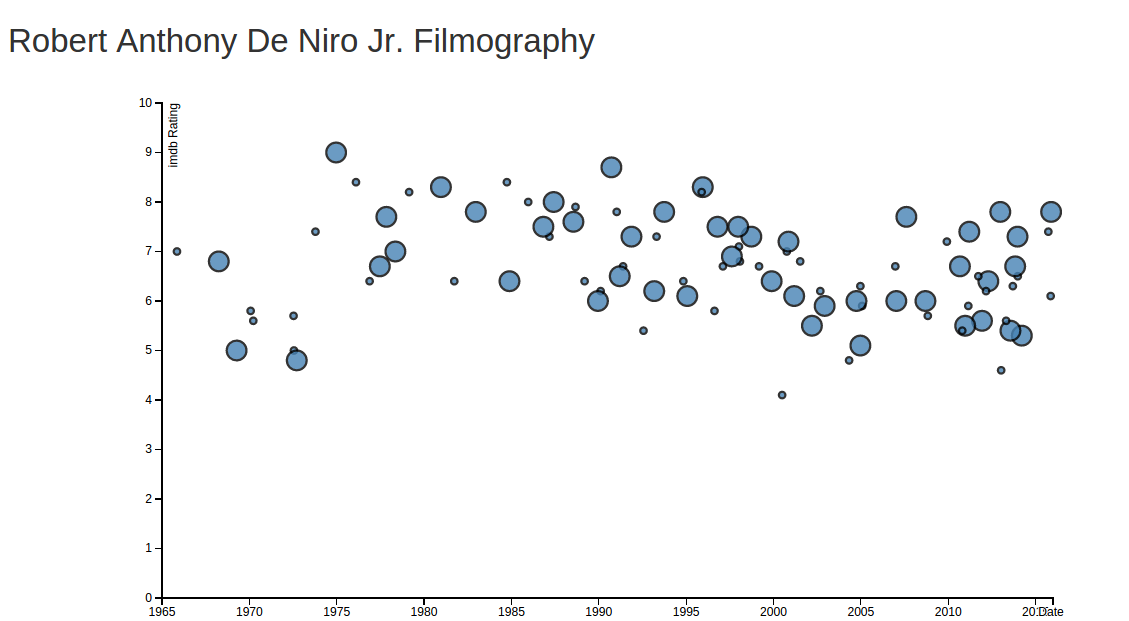
\includegraphics[width=.7\linewidth]{images/Deniro_timeline.png}
				  \caption{We've seen better times.}
\end{figure}\label{fig:deniro}


\subsubsection{Genre Visualization}

	\begin{figure}[h!]
		\centering
		\begin{subfigure}[t]{.5\textwidth}
		  \centering
		  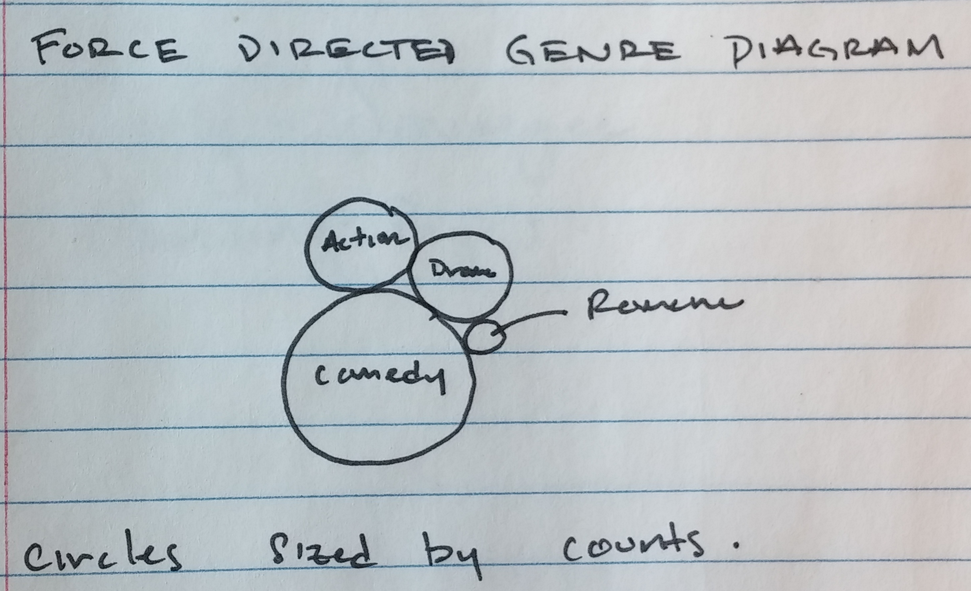
\includegraphics[width=\linewidth]{images/genreVis_crop.png}
		  \caption{Original design sketch}
		  \label{fig:sub1}
		\end{subfigure}%
		\begin{subfigure}[t]{.8\textwidth}
		  \centering
		  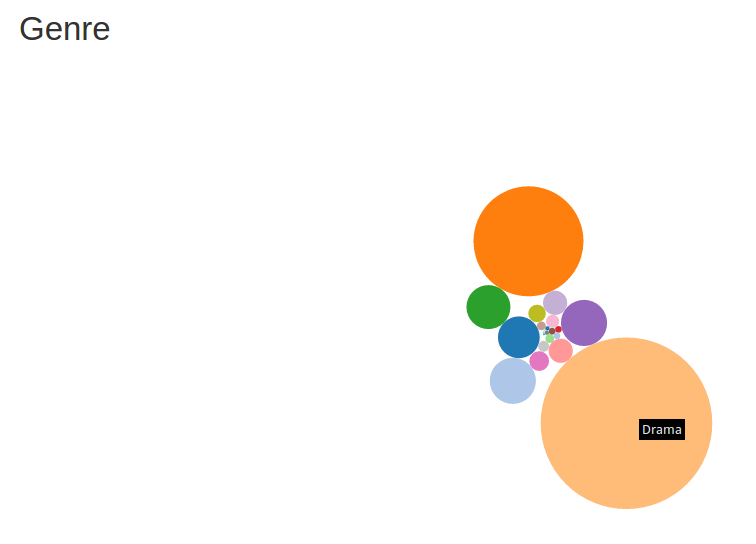
\includegraphics[width=.7\linewidth]{images/genreVis.png}
		  \caption{Current implementation}
		  \label{fig:sub2}
		\end{subfigure}%
		\caption{Genre visualization development}
		\label{fig:genreVis}
	\end{figure}

\subsubsection{Parallel Axis Coordinate Visualization}
	
	\begin{figure}[h!]
		\centering
		\begin{subfigure}[t]{.5\textwidth}
			  \centering
			  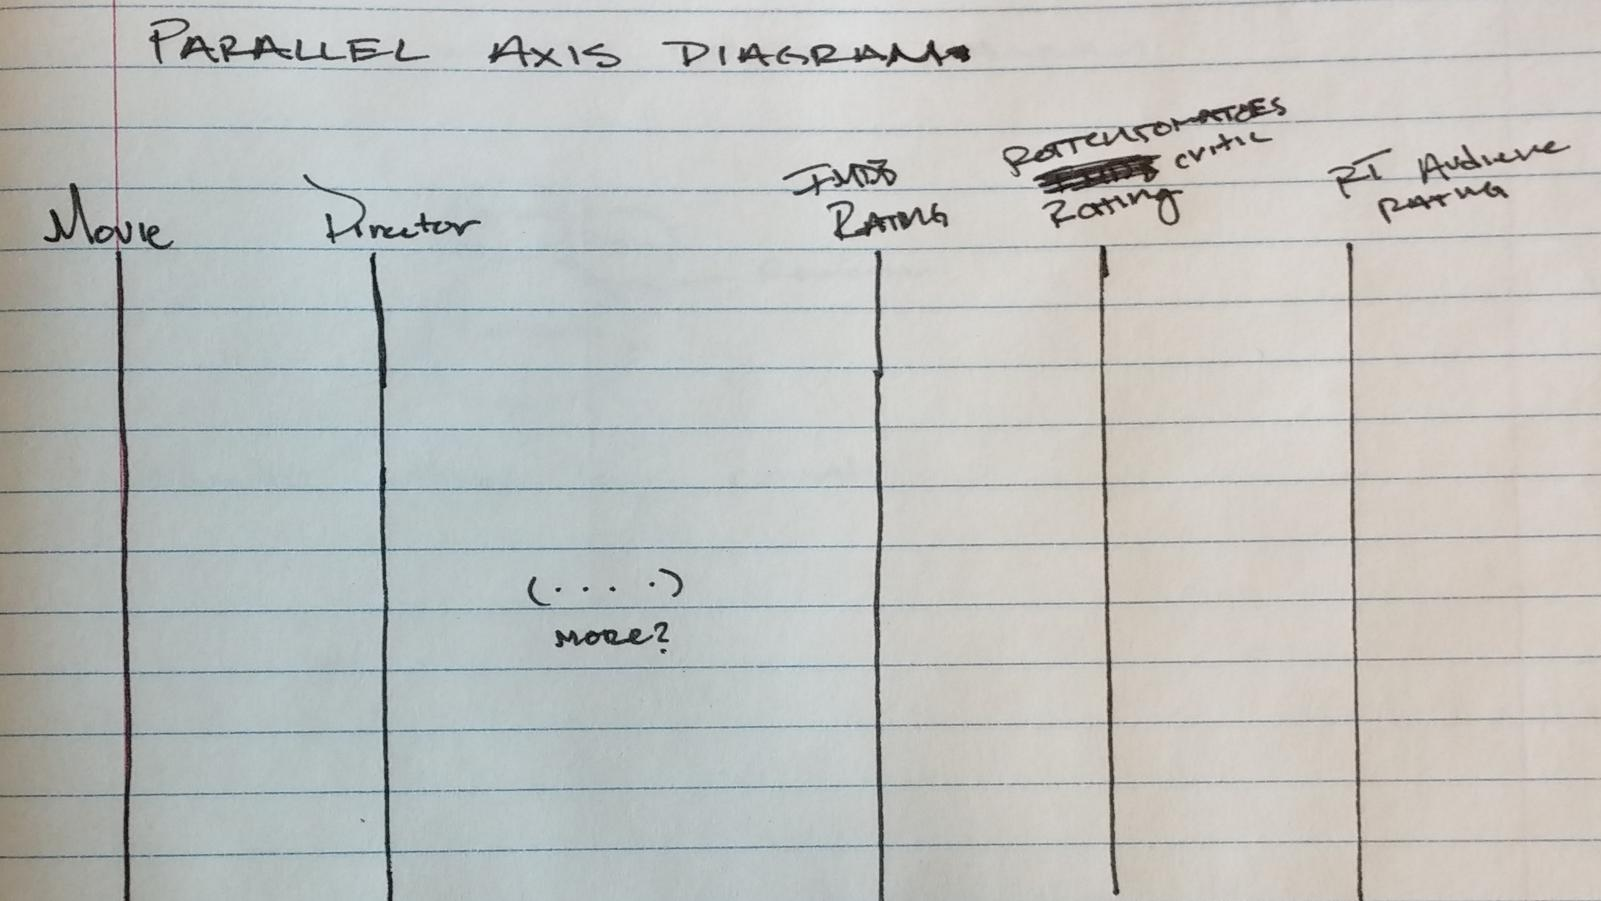
\includegraphics[width=\linewidth]{images/parallel_crop.jpg}
			  \caption{Original design sketch}
			  \label{fig:sub1}
		\end{subfigure}%
		\begin{subfigure}[t]{.8\textwidth}
			  \centering
			  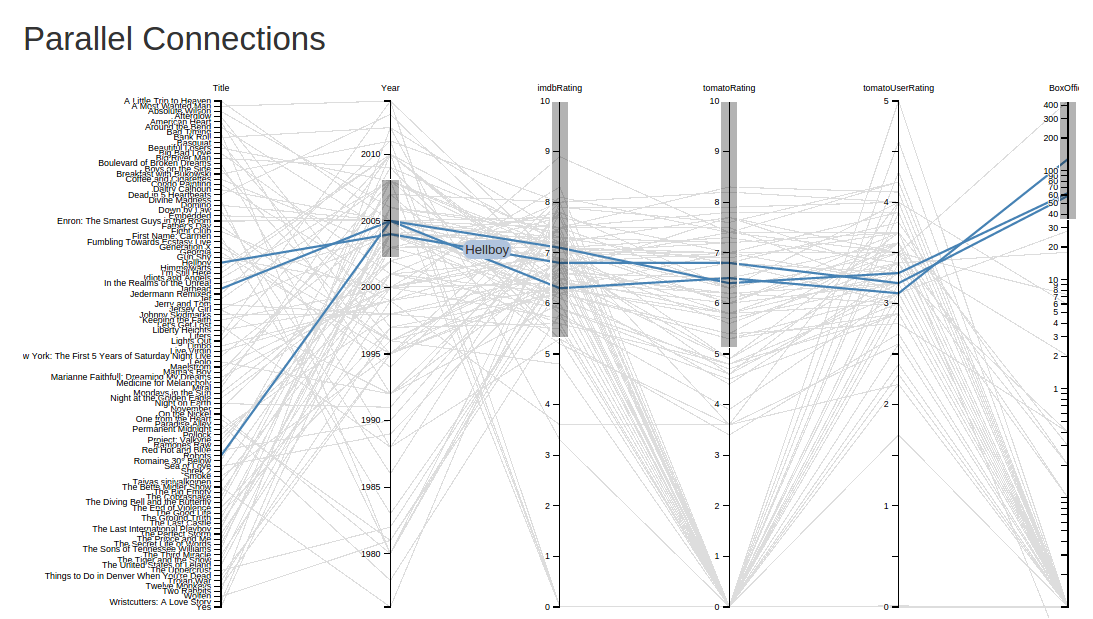
\includegraphics[width=.7\linewidth]{images/parallelAxisCoordVis.png}
			  \caption{Current implementation}
			  \label{fig:sub2}
		\end{subfigure}%
		\caption{Parallel Axis Coordinate visualization development}
		\label{fig:parallelAxisCoordVis}
	\end{figure}

\newpage

\section{Project Feedback} \label{sec:Projcet Feedback}

After we settled on our design and project implementation, we had the opportunity to present a ``sales pitch"  for Curly-Squeegee to another project team to get their feedback.  We met with Phil Cutler, Ariel Herbert-Voss, and Ian Sohl of the "Legion Profiling Visualization" team. They provided the following feedback:

\begin{itemize}
	\item \textbf{Phil Cutler} (u0764757@utah.edu)
	
	Provided good feedback and constructive criticism. Raised concerns about Parallel axis plot readability in the limit of a long, active acting career as well as a lack of information on new actors. Liked the idea of the filmography visualization, but recommended using bar charts as opposed to circles anchored to a timeline. He thought it was a neat idea, but did not see it's utility. He admitted he does not like watching movies.
	
	
	\item \textbf{Ariel Herbert-Voss} (u0591949@utah.edu)
	
	Overall very positive and excited reaction. she loved the parallel axis plot idea and also agreed with Phil that a bar chart for the filmography timeline would be more effective. She suggested scaling bars either by film rating or number of films in a given period (for a drill-down style barchart), as well as shading a given bar to convey additional information. Ariel is a film buff and saw a great deal of utility in this visualization
	
	\item \textbf{Ian Sohl} (u0445696@utah.edu)
		No additional feedback beyond what Phil and Ariel had to suggest.
\end{itemize}

\newpage

\section{Team Evaluation}

\textit{Brian Kimmig}: Brian was responsible for the API calls, data collection, and database wrangling. His experience as a web developer was very helpful for making this portion of the project go very smoothly. Brian also created the project framework, and parallel coordinate view.

\textit{Jimmy Moore}: Jimmy was the lead scribe for the group and was responsible for project documentation including the proposal and process book. He also coded the Actor photo and display box features and filmography timeline visualization.


\end{document}